\section{Concepts Implemented in EASAL}
In this section we discuss the major concepts implemented in \EASAL.

\subsection{Exploration}
\figref{fig:algorithm} gives an overview of how sampling and exploration is done in \EASAL.
It involves stratification, Cayley sampling and, convex parameterization, each of which is explained here.
\begin{figure}
\centering
\includegraphics[width=\textwidth] {\fig/Algorithm.png}
\caption{Algorithm for generating and exploring the atlas}
\label{fig:algorithm}
\end{figure}

\subsubsection{Stratification}
Startification stores and labels regions of the
configuration space represented by an atlas. The regions of the atlas are stored as nodes of a
directed acyclic graph (\figref{fig:natlas} and \figref{fig:flips}), whose
edges represent immediate containment or reachability. Each region of the
atlas is identified by an \textit{activeConstraintGraph} $G_H$ where $H$
is the set of active constraints. A newly discovered $G_H$ is tested to ensure
that it is not already present in the current \emph{atlas}. Only if $G_H$ is
new the region is further explored; by default, this is done depth first. New
active constraints and regions are added individually by sampling the space at
a user specified level of refinement.

\subsubsection{Cayley Sampling}
We sample the active constraint regions via Cayley parameter grid sampling 
to define the grid. In addition we use binary search near
the boundary to discover lower dimensional boundary regions where new
constraints become active as described under `Detect Active Constraint'. We
determine the parameter set $F$ of the active constraint graph that yields a
partial 3-tree. We then compute the range of $F$ for the active constraint
region.

\subsubsection{Convex Parametrization}
The parameters $F$ of an active constraint graph are selected so as to form a maximal
3-tree to leverage the convex parametrization
theory~\cite{Gao}. The algorithm works by searching a superset of the active
constraints of the graph from the list of complete 3-trees in
\figref{fig:3-trees}. For this purpose a look-up table is created, that holds
all complete 3-trees. Searching is done among all isomorphisms of the graphs of
complete 3 trees. If a superset is found then the edges in that graph (except
the active constraints) will be used as the parameter set.

\subsection{A Priori Boundary Detection}
Boundary detection is done to make sure that sampling does not go beyond the feasible
region. Some of these boundary detection is done prior to the Cartesian realization
of a Cayley point and some are done after the realization. The boundaries detected
a priori include the tetrahedral inequalities and the steric constraints of the
atoms involved in the active constraints.


\subsubsection{Detect Tetrahedral Bounds (Cayley-Menger inequalities): Chart Range Computation}
If Convex Cayley parametrization theory is
applicable to the active constraint graph, then the chart that is defined by
the set of Cayley points traced out by the Cayley parameters happens to be
convex. In other words, the active constraint graph has a convex Cayley
configuration space if it is a partial 3-tree. Then we need to compute the
bounds of the convex region where the sampling occurs and prevent the sampling
from going beyond the feasible region. Finding bounds for each non-edge has two cases
and the range computation for each of these cases is handled as follows:
\begin{itemize}
		\item When there is only one parameter in a tetrahedron and all the
				other edges are fixed, the range of that parameter can be
				computed by the intersection of the triangular and tetrahedral
				inequalities.
		\item If there is more than one unfixed parameter in the tetrahedron,
				then the range of all parameters except one will be computed
				through triangular inequalities and fixed by assigning a value
				within their range. Then the range of the one remaining
				parameter will be computed as in the first case through both
				triangular and tetrahedral inequalities. Since the range of
				the parameter is affected by the previously fixed parameters,
				range computation of the unfixed parameter is required
				for every iteration/assignment of fixed parameters.
\end{itemize}

Fixing a non-edge requires the range
computation for the non-fixed parameter that takes place in the same
tetrahedron. The order in which this is done has an effect on the efficiency
of sampling~\cite{ugandhar}. We pick the parameters in the order
that gives the best efficiency.

\subsubsection{Detect Active Constraint}
Detects a newly active constraint and a new
region of the stratification in a smaller dimensional stratum. \EASAL~relies on
Cayley parameter grid sampling to find the children of each active constraint
region and uncover the topology of the atlas by exhaustively exploring
boundaries with a certain step size. When a new active constraint is detected
via binary search described under `Cayley Sampling', the regions of its children
are recursively sampled and explored.

However, boundary detection is not guaranteed by Cayley parameter grid sampling alone. The
threshold may not be large enough to allow the Constraint Check algorithm to
define a close by atom pair to be a distance constraint, i.e., edge of the
active constraint graph. Furthermore, neighboring Cayley points may be in
violation of steric, hard sphere, or global constraints. As a result, the boundary
region would be missed since it is located in between a feasible point and a
point violated by sterics. Exploration (by the way of binary search) is
required to find any additional constraints that restrict the region, e.g.,
steric constraints that render a configuration infeasible.

\begin{figure}
\centering
\includegraphics[scale=0.35] {\fig/partial3tree_new.png}
\includegraphics[scale=0.35] {\fig/partial3tree_new_2.png}
\caption{All 3-tree active constraint graphs for $k = 2$ rigid bodies in $R^3$.
It should be noted that the vertices on the left and the right of this graph
form a complete graph (edges not shown) since the atoms on each node belong to a
rigid unit.  The label $m_1$ $m_2$ below each active constraint graph indicates
that $m_1$ atoms in $M_1$ are connected to $m_2$ atoms in $M_2$ . Solid edges
indicate pairs whose distance is fixed matching their Lennard-Jones potential.}
\label{fig:3-trees}
\end{figure}
\subsection{Cartesian Realization}
We find Cartesian realizations in 3D, and we have only
2 degrees of freedom per dimension. Therefore, when we fix 6 active constraints,
we are out of degrees of freedom. Hence, atlas nodes are always 5D or lower.
To find the Cartesian realization we add one atom at a time using distances
from already realized atoms to get a partial 3-tree. This gives us a convex
space and in addition makes finding a realization easier than the general
Cartesian realization problem. For nodes of dimensions 3 and higher, we are
always guaranteed to get a convex region. For 1D and 2D regions, i.e., when 4 or
5 constraints are active, we sometimes end up with a non-convex region, we drop
a constraint and explore a higher dimensional region using ray tracing to
compute the Cartesian realization.


\subsection{A Posteriori Boundary Detection}
After the realization, we can detect certain other boundaries which include
detecting predefined interactions, detecting steric constraints of molecules
not a part of the active constraints and detecting global angle constraints.

\begin{figure}
\subfigure[Cayley points in the Cayley space view. On the left, we see all the
Cayley points and on the right we see the boundary
points shown differently.]{\includegraphics[width=60mm]{\fig/space.eps}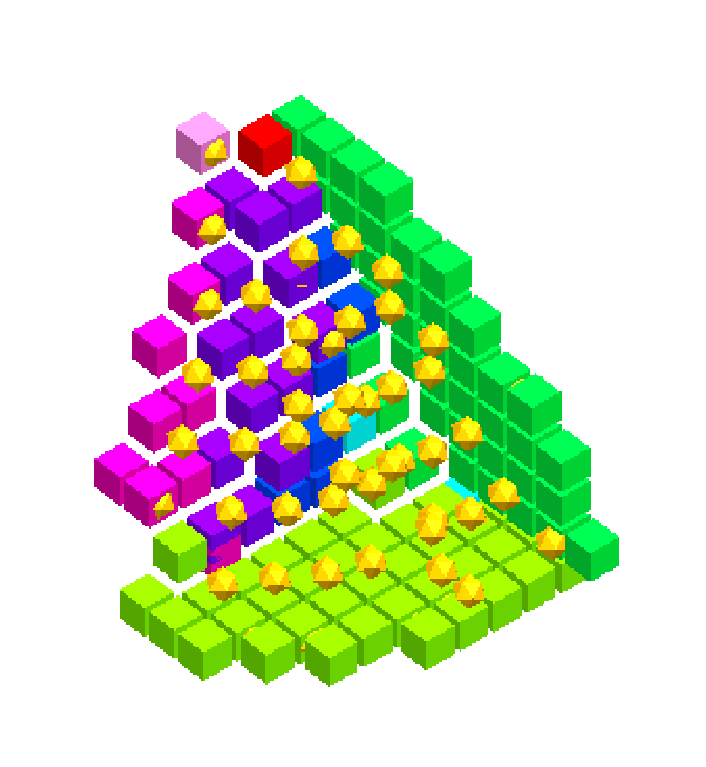
\includegraphics[width=60mm]{\fig/spaceboundaries.eps}}
\hskip0.01\linewidth
\subfigure[Cartesian sweep view. On the left we see all the Cartesian realizations and on
the right we see the Cartesian realizations along different boundaries in different
colors.]{\includegraphics[width=60mm]{\fig/sweepview.eps}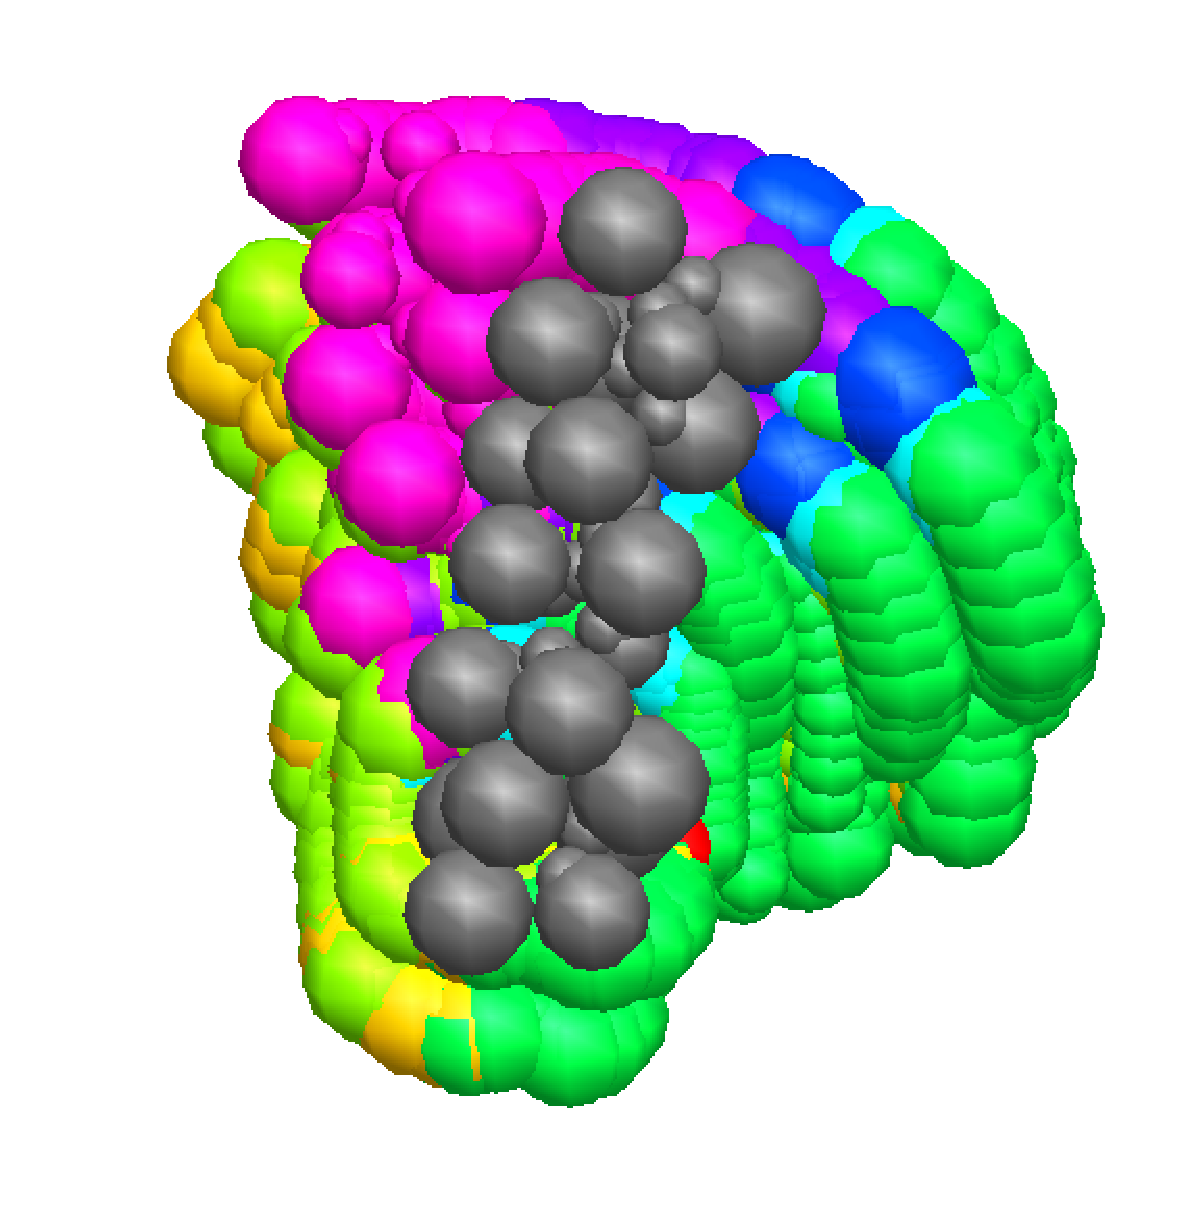
\includegraphics[width=60mm]{\fig/sweepboundaries.eps}}
\label{ImprovedChildSampling}
\caption{An active constraint region showing (a) the Cayley points (b) the Cartesian realization.}
\end{figure}
